\autobookmark
\begin{frame}[t]{A fast simulation enables simulation of the ASE-temperature equilibrium}
  \begin{columns}[T]
    \begin{column}{.5\textwidth}
      \myonly{1}{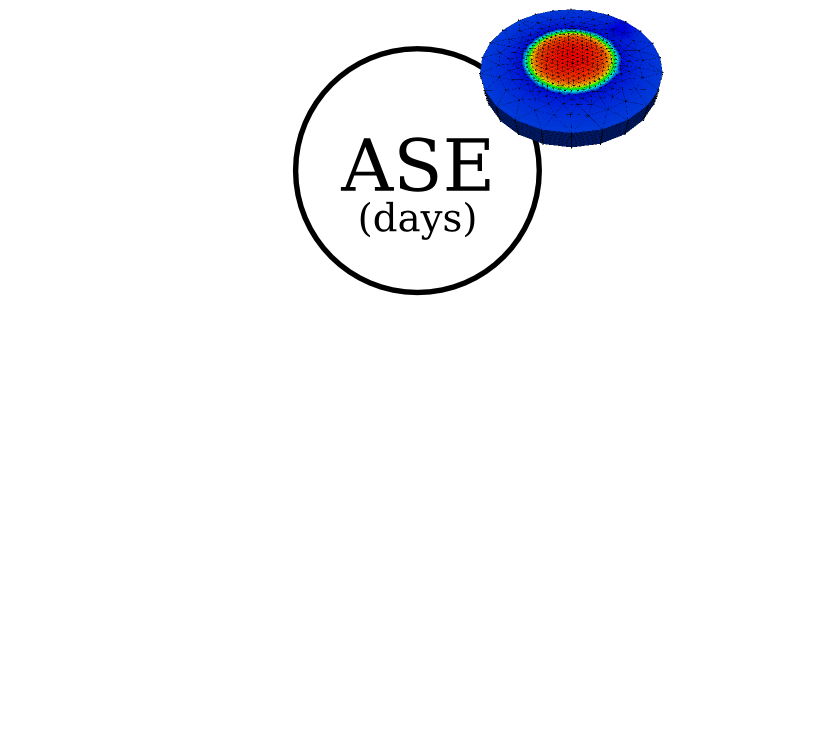
\includegraphics[width=.5\paperwidth]{graphics/ASE_temperature_equilibrium1.png}}
      \myonly{2}{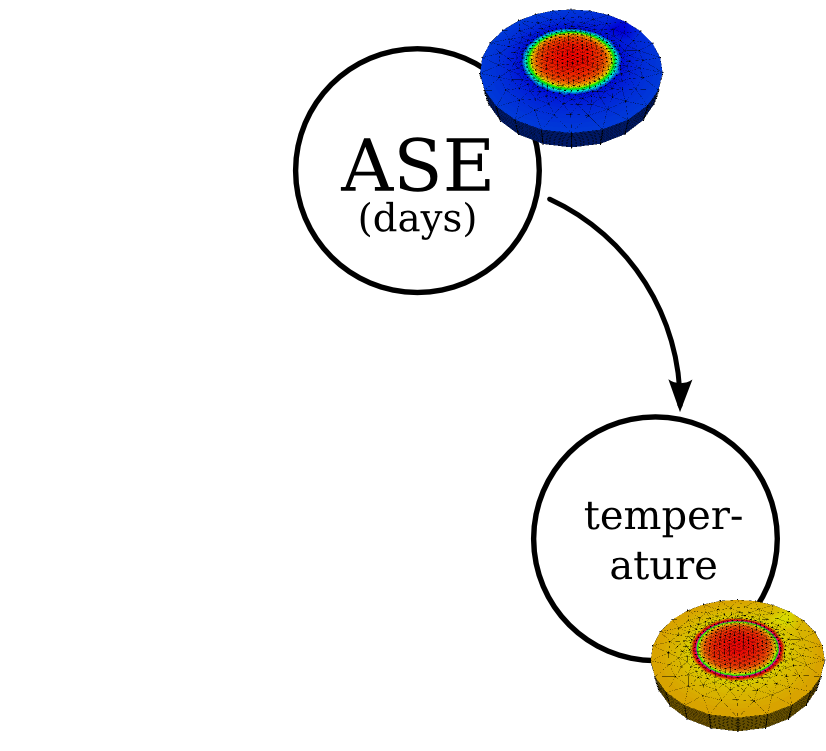
\includegraphics[width=.5\paperwidth]{graphics/ASE_temperature_equilibrium2.png}}
      \myonly{3-4}{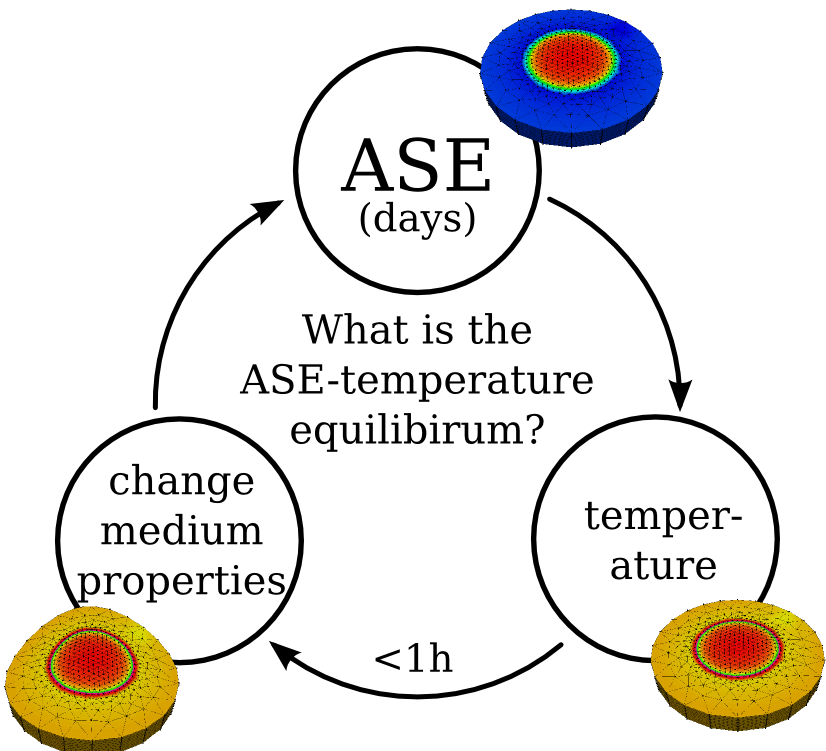
\includegraphics[width=.5\paperwidth]{graphics/ASE_temperature_equilibrium3.png}}
    \end{column}
    \begin{column}{.5\textwidth}
      \begin{itemize}
          \myuncover{2}{4}{
          \item The energy from ASE increases the temperature of the gain medium
          }
          \myuncover{3}{4}{
          \item The change in temperature creates mechanical and optical
            changes, which influence the ASE
          }
          \myuncover{4}{4}{
          \item The calculation of ASE is time-consuming, making an iterative
            computation very costly
          }
      \end{itemize}
    \end{column}
  \end{columns}
\end{frame}
